\chapter{Nyelvtanok és osztályozásuk}

\section{Nyelvek definiálási módjai}

\begin{enumerate}
	\item Felsorolással: $ L := \{ \texttt{pa}, \texttt{ta}, \texttt{ka} \} $.
	\item Logikai formulával (invariánssal):
	$ L := \{ \texttt{a}^n\texttt{b}^n \mid n \in \mathbb{N} \} $.
	\item Strukturális rekurzióval: megszámlálhatóan végtelen nyelveken végrehajtunk véges számú elemi műveletet. \[ L := \{ \texttt{ab}\}^* \{ \texttt{cd} \}^{} \]
	\item Algoritmussal
	\item Matematikai gépekkel (automatákkal)
	\item Produkciós rendszerekkel (szabályokkal)
\end{enumerate}

A továbbiakban a produkciós rendszerekkel fogunk részletesebben foglalkozni.

\section{Nyelvtanok}

\begin{tcolorbox}
	\begin{definition}[Nyelvtan]
		\textbf{Nyelvtan}nak (vagy \textbf{grammatiká}nak) nevezzük az alábbi négyest:
		\[ G := ( N, T, P, S), \] ahol
		\begin{itemize}
			\item $N$ a \textbf{nemterminális jelek} halmaza,
			\item $T$ a \textbf{terminális jelek} halmaza (ábécé),
			\item $P$ a \textbf{produkciós szabályok} halmaza,
			\item $S$ a \textbf{startszimbólum} (vagy kezdőszimbólum).
		\end{itemize}
	\end{definition}
\end{tcolorbox}

Kiemelünk pár tulajdonságot, amik a nyelvtan összetevőire teljesülnek.
\begin{itemize}
	\item $N \cup T = \emptyset$, azaz a nemterminálisok és terminálisok halmaza diszjunktak.
	\item $S \in N$, azaz a startszimbólum egy nemterminális jel.
	\item $P$ elemeit \textbf{produkciós szabályok}nak nevezzük, melyeket az alábbi módon írunk le:
	\[ (p,q) \in P ~ \Longleftrightarrow ~ p \longrightarrow q \in P. \]
	\begin{itemize}
		\item A szabály bal oldalának alakja: $p \in (T \cup N)^* N(T \cup N)^*$. \textit{Jelentése}: legalább egy nemterminálisnak muszáj szerepelnie a szabály bal oldalán.
		\item A szabály jobb oldalának alakja: $q \in (T \cup N)^*$.
		\item A szabály két oldalát a ``$\longrightarrow$'' jellel választjuk el.
		\item \framebox{A $(T\cup N)^*$ halmaz elemeit \textbf{mondatformá}knak nevezzük}. A fogalom azért szükséges, ugyanis meg akarjuk különböztetni, hogy mikor beszélünk ``tisztán'' szóról és mikor terminálisok és nonterminálisok vegyes véges sorozatáról.
	\end{itemize}
\end{itemize}

\begin{tcolorbox}
	\begin{definition}[Nyelvtan által generált nyelv]
		Legyen $G := (N,T,P,S)$. Ekkor a $G$ nyelvtan által generált nyelv azon szavak halmazát jelenti, melyek \textbf{közvetlenül vagy közvetetten levezethetők a $G$-ből}, vagyis 
		\[ L(G) := \left\{ u \in T^* \setdivbar S \genword{G}{*} u \right\}. \]
	\end{definition}
\end{tcolorbox}

Pár szót a jelölésről. A $*$ arra utal, hogy mennyi lépésben tudunk eljutni az $S$ kezdőszimbólumból az $u$ szóig. Véges sok lépésszámot kell jelentsen. Akár konkrét értéket is megadhatunk. A $G$ csupán arra utal, hogy a $G$ nyelvtan generálja a szóban forgó szót. Ha a kontextusból egyértelmű, akkor elhagyhatjuk.

Továbbá figyeljük meg, hogy eltérő nyilat ($\Longrightarrow$) használunk arra, amikor mondatformából vezetünk le egy szót. Az előző eset ($\longrightarrow$) csupán a produkciós szabály jobb és bal oldalának elválasztására szolgált.

A definícióban szerepelt olyan megfogalmazás, hogy közvetetten, illetve közvetlenül levezetünk egy szót a startcsúcsból. A levezetés ezen két fajtáját itt definiáljuk.

\begin{tcolorbox}
	\begin{definition}[Közvetlen levezetés]
		Legyen $G := (N,T,P,S)$ egy adott nyelvtan, valamint legyen $u,v \in (T\cup N)^*$ két mondatforma. Azt mondjuk, hogy a \textbf{$v$ mondatforma közvetlenül levezethető az $u$ mondatformából}, ha 
		\[ \exists u_1, u_2 \in (T\cup N)^*, \exists \prodrule{x}{y} \in P : u = u_1 x u_2 \land v = u_1 y u_2. \] Jelölése: $\boxed{u \genword{G}{} v}$.
	\end{definition}
\end{tcolorbox}

\begin{tcolorbox}
	\begin{definition}[Közvetett levezetés]
		Legyen $G := (N,T,P,S)$ egy adott nyelvtan, valamint legyen $u,v \in (T\cup N)^*$ két mondatforma. Azt mondjuk, hogy a \textbf{$v$ mondatforma közvetetten levezethető az $u$ mondatformából}, ha 
		\[ \exists k \in \mathbb{N}, \exists x_0, x_1, \dots, x_k \in (T\cup N)^*, u = x_0 \land v = x_k, \forall i \in [0 \dotdot k-1]: x_{i} \genword{G}{} x_{i+1}. \] Jelölése: $\boxed{u \genword{G}{*} v}$.
	\end{definition}
\end{tcolorbox}

Szavakban: létezik egy $k$ elemből álló mondatformák sorozata, melynek legeleje az $u$ és legvége a $v$. Ezek között egyesével haladva közvetlenül levezethetők az egyes mondatformák úgy, hogy a sorozatban a soron következőbe jutunk el.

\begin{tcolorbox}
	\begin{definition}[Nyelvek ekvivalenciája]
		Legyen $G_1, G_2$ két nyelvtan.
		\begin{itemize}
			\item $G_1$ és $G_2$ \textbf{ekvivalensek}, ha $\boxed{L(G_1) = L(G_2)}$ .
			\item $G_1$ és $G_2$ \textbf{kvázi-ekvivalensek}, ha $\boxed{L(G_1) \setminus L_\emptyword = L(G_2) \setminus L_\emptyword}$ , azaz csak az üres szó generálásában térnek el.
		\end{itemize}
	\end{definition}
\end{tcolorbox}

\begin{tcolorbox}
	\begin{theorem}
		Nem minden nyelv írható le nyelvtannal.
	\end{theorem}
\end{tcolorbox}

\section{A Chomsky-féle grammatikatípusok}

\begin{tcolorbox}
	\begin{definition}[Chomsky-féle grammatikatípusok]
		A $G =(N,T,P,S)$ nyelvtan $i$-típusú $(i =0,1,2,3)$, ha $P$ szabályhalmazára teljesülnek a következők:
		\begin{enumerate}
			\item[0.] \textbf{típus} $(i=0)$ -- Nincs korlátozás.
			\item \textbf{típus} $(i=1)$ -- \textbf{környezetfüggő nyelvtan}: \\ $P$ minden szabálya 
			$\boxed{\prodrule{u_1Au_2}{u_1vu_2}}$ alakú, ahol $u_1,u_2,v \in (N \cup T)^*$, $A \in N$, és $v \neq \emptyword$, kivéve az $\prodrule{S}{\emptyword}$ alakú szabályt, de ekkor $S$ nem fordul elő egyetlen szabály jobboldalán sem.\footnote{Ezt "\textit{Korlátozott $\emptyword$-szabály}”-nak, röviden: KES-szabálynak hívjuk.}
			\item \textbf{típus} $(i =2)$ -- \textbf{környezetfüggetlen nyelvtan}: \\ $P$ minden szabálya $\boxed{\prodrule{A}{v}}$ alakú, ahol $A \in N$, $v \in (N \cup T)^*$.
			\item \textbf{típus} $(i =3)$ -- \textbf{reguláris nyelvtan}: \\ $P$ minden szabálya vagy $\boxed{\prodrule{A}{uB}}$ vagy $\boxed{\prodrule{A}{u}}$ alakú $(A,B \in N, u \in T^*)$.
		\end{enumerate}
	\end{definition}
\end{tcolorbox}

Az $i$-típusú nyelvtanok vagy grammatikák halmazát $\boxed{\mathcal{G}_i}$  -vel jelöljük. A grammatikák alakjából következik, hogy 
\begin{flalign*}
	& \mathcal{G}_i \subseteq \mathcal{G}_0 ~~~ (i = 1, 2, 3). \\
	& \mathcal{G}_3 \subseteq \mathcal{G}_2.
\end{flalign*}

\begin{tcolorbox}
	\begin{definition}
		Egy $L$ nyelvet $i$-típusúnak nevezünk $(i \in \{0, 1, 2, 3\})$, ha létezik olyan $i$-típusú grammatika, ami az $L$ nyelvet generálja, azaz  \[ \exists G \in \mathcal{G}_i : L(G) = L. \]
	\end{definition}
\end{tcolorbox}

Az $i$-típusú nyelvek halmazát -- nyelvcsaládját, nyelvosztályát -- jelölje $\mathcal{L}_i$, azaz
\[ \mathcal{L}_i := \left\{ L \text{ nyelv} \setdivbar \exists G  \in \mathcal{G}_i : L(G) = L \right\} ~~~~ (i = 0, 1, 2, 3). \]

\begin{tcolorbox}
	\begin{theorem}[Chomsky-féle hierarchia]
		\[ \mathcal{L}_3 \subseteq \mathcal{L}_2 \subseteq \mathcal{L}_1 \subseteq \mathcal{L}_0. \]
		\begin{center}
			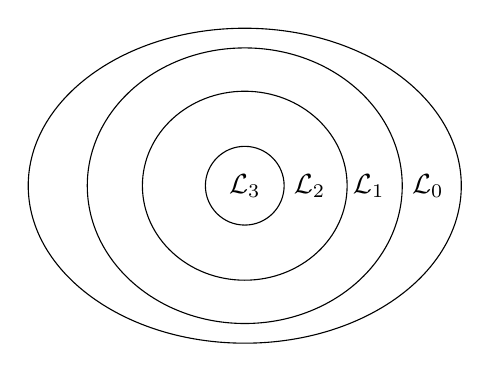
\begin{tikzpicture}
				% Sets
				\draw (0,0) ellipse (2.75cm and 2cm) node {$\mathcal{L}_3$};
				\draw (0,0) ellipse (2cm and 1.75cm) node[right=0.5cm] {$\mathcal{L}_2$};
				\draw (0,0) ellipse (1.3cm and 1.2cm) node[right=1.25cm] {$\mathcal{L}_1$};
				\draw (0,0) ellipse (0.5cm and 0.5cm) node[right=2cm] {$\mathcal{L}_0$};
			\end{tikzpicture}
		\end{center}
	\end{theorem}
\end{tcolorbox}

\textit{\textbf{Megjegyzés}}. A tartalmazásnak $\mathcal{L}_2 \subseteq \mathcal{L}_1$ része nem triviális az 1-es típusú nyelvek (nyelvtanok) kínos definíciója miatt.

A tételnek létezik az \textbf{erősebb változata}, mely valódi tartalmazást állít:
\[ \mathcal{L}_3 \subset \mathcal{L}_2 \subset \mathcal{L}_1 \subset \mathcal{L}_0. \]

Figyeljük meg, hogy a Chomsky-féle hierarchia \textbf{nyelvcsaládokra} és \textbf{nem nyelvtanokra} vonatkozik. Emiatt
\[ \mathcal{G}_3 \subseteq \mathcal{G}_2 \subsetneq \mathcal{G}_1 \subseteq \mathcal{G}_0. \]
Ha a 2-es típusú szabályoknál is kikötnénk, hogy $v \neq \emptyword$, akkor igaz lenne a tartalmazás, és akkor triviálisan igaz lenne a nyelvcsaládokra is tartalmazás.

Ha ugyanazon nemterminálishoz több szabály tartozik, akkor tömörebben is felírhatjuk a rá vonatkozó szabályokat az alábbi módon:
\[ \prodrule{S}{\emptyword \mid \texttt{a}S\texttt{b} \mid SS}, \]
ahol a ``~|~'' jelek amolyan ``\textit{vagy}'' jelentéssel bíró elválasztók. Ezt használja ki a \textbf{Backus--Naur-jelölés} (angolul \textbf{Backus--Naur-form}, röviden \textbf{BNF}), melyet a programozási nyelvek szintaxisának felírásához szoktak használni. Például ugyanez a nyelv BNF-fel felírva:
\[ \texttt{<start> ::= $\emptyword$ | a <start> b | <start> <start>}, \]
ahol a \fbox{\texttt{<}, \texttt{>}} jelek olyan \textit{metaszimbólumok}, melyekkel meg lehet címkézni az egyes nemterminálisokat. A \fbox{\texttt{::=}} felel meg a $\longrightarrow$ jelölésnek.

Egy egyszerű példa, ami néhány magyar mondat generálására képes. Az egyszerűség kedvéért feltesszük, hogy egyetlen terminális jelből áll a \texttt{macska}, \texttt{kutya}, stb. szavunk.
\begin{align*}
	&\texttt{<mondat>} & \texttt{ ::= } &\texttt{<alany> <állítmány> .} \\
	&\texttt{<alany>} & \texttt{ ::= } &\texttt{<névelő> <főnév> | <névelő> <melléknév> <főnév>} \\
	&\texttt{<névelő>} & \texttt{ ::= } &\texttt{A | Egy} \\
	&\texttt{<főnév>} & \texttt{ ::= } &\texttt{macska | kutya} \\
	&\texttt{<melléknév>} & \texttt{ ::= } &\texttt{bozontos | kerge} \\
	&\texttt{<állítmány>} & \texttt{ ::= } &\texttt{eszik | iszik | alszik}
\end{align*}

\section{Nyelvtani transzformációk}

Ahogyan korábban be lett vezetve, B szakirányon az elmélet leginkább a fordítóprogramok írásához legszükségesebb ismereteket adja át, emiatt a most következőket csak 3-as típusú nyelvtanokra, nyelvekre fogalmazzuk meg, ugyanis ezen nyelvek teszik lehetővé, hogy 

\begin{tcolorbox}
	\begin{definition}[Nyelvtani transzformáció]
		A nyelvtani transzformáció olyan eljárás, amely egy $G$ grammatikából egy másik $G'$ grammatikát készít.
	\end{definition}
\end{tcolorbox}

\begin{tcolorbox}
	\begin{definition}[Ekvivalens nyelvtani transzformáció]
		Ekvivalens nyelvtani transzformációról beszélünk, ha minden $G$ nyelvtanra és az ő $G'$ transzformáltjára igaz, hogy $L(G) = L(G')$.
	\end{definition}
\end{tcolorbox}

\subsection{Epszilon-mentesítés ($\emptyword$-mentesítés)}

A fordítóprogramok szempontjából fontos transzformációnk az ún. \textbf{\textit{$\emptyword$-mentesítés}}.

\begin{tcolorbox}
	\begin{theorem}[$\emptyword$-mentesítés]
		Minden $G = (N,T,P,S)$ \textbf{környezetfüggetlen} (2-es típusú) nyelvtanhoz megkonstruálható egy vele ekvivalens $G' = (N', T', P', S')$ \textbf{környezetfüggetlen} nyelvtan úgy, hogy $P'$-ben nincs $\prodrule{A}{\emptyword}$ alakú szabály, kivéve ha $\emptyword \in L(G)$, mert akkor $\prodrule{S'}{\emptyword} \in P'$, de ekkor $S'$ nem szerepelhez szabály jobb oldalán.
		
		Formális(abb)an:
		\[ \forall G = (N, T, P, S) \in \mathcal{G}_2 , \exists G' = (N', T', P', S') \in \mathcal{G}_2, L(G') = L(G): \]
		\begin{itemize}
			\item $\emptyword \notin L(G) \Longrightarrow$ nincs olyan szabály $P'$-ben, amely ``$\prodrule{A}{\emptyword}$'' alakú lenne,
			\item $\emptyword \in L(G) \Longrightarrow \prodrule{S'}{\emptyword} \in P'$, de ekkor $S'$ nem szerepelhet más szabály jobb oldalán.
		\end{itemize}
	\end{theorem}
\end{tcolorbox}

~\\[-2.5em]

\begin{mdframed}
	\textbf{\textit{Bizonyítás}}. A bizonyítás több lépésből áll.
	\begin{enumerate}[1.)]
		\item Határozzuk meg, hogy mely nemterminálisokból vezethető le az üres szó!
		\[ H := \left\{ A \in N \setdivbar A \genword{G}{*} \emptyword \right\}. \]
		Ehhez definiáljuk az alábbi $H_i$ halmazokat ($i \geq 1$):
		\begin{flalign*}
			H_1 & := \left\{ A \in N \setdivbar \exists \prodrule{A}{\emptyword} \in P \right\}, \\
			H_{i+1} & := H_i \cup \left\{ A \in N \setdivbar \exists \prodrule{A}{w} \in P \land w \in H_i^* \right\}.
		\end{flalign*}
		Ebből nyilvánvalóan teljesül a következő összefüggés:
		\[ H_1 \subseteq H_2 \subseteq \dots \subseteq H_i \subseteq H_{i+1}. \] 
		Mivel $\forall i \geq 1: H_i \subseteq N$ és $N$ véges halmaz, ezért egy $k \in \mathbb{N}$ indextől kezdődően biztosan azonosak lesznek a halmazok, azaz \[ \exists k \in \mathbb{N}, \forall i \in \mathbb{N} : H_k = H_{k+i}. \] Így legyen $H := H_k$.
		
		(\textit{Megjegyzés}. Ennek a részletesebb belátása az [1.] jegyzet 16. oldalán elolvasható.)
		
		Ekkor látható, hogy 
		\[  A \in N \land A \genword{G}{*} \emptyword ~~ \Longleftrightarrow ~~ A \in H. \] 
		Ennek következménye, hogy \[ \emptyword \in L(G) ~~ \Longleftrightarrow ~~ S \in H. \]
		
		\item Alakítsuk át $H$ ismeretében a grammatika szabályait a kellő alakúra.
		\begin{enumerate}
			\item $\boxed{S \notin H}$ : $\prodrule{A}{v'}\in P'$ akkor és csak akkor, ha $v' \neq \emptyword$ és $\exists \prodrule{A}{v}\in P$ úgy, hogy $v'$-t a $v$-ből úgy kapjuk meg, hogy elhagyunk nulla vagy több $H$-beli nemterminálist $v$-ből.
			\item $\boxed{S \in H}$ : A korábbi szabályhoz hozzávesszük még a következő két szabályt: 
			\[ \prodrule{S'}{\emptyword \mid S} \] ahol $S' \notin N$ és $S'$ a $G'$ nyelvtan új startszimbóluma. $\square$
		\end{enumerate}
	\end{enumerate}
\end{mdframed}

\textbf{\textit{Megjegyzés}}. A tételt ugyan 2-es típusú nyelvtanokra mondtuk ki, de 3-as típusúakra is tökéletesen működik.

\subsection{Nyelvek normálformája}

A négy nyelvtani típusból háromnak létezik ún. \textbf{normálformá}ja. Ezek a normálformák olyan alakra hozzák az adott típusú nyelvtanok szabályait, melyek egyrészt könnyebben felismerhetővé, egyértelműbbé teszik a típusát, másrészt ez az alak nagy segítségünkre válik, amikor az automatákkal is elkezdünk foglalkozni. Eme ekvivalens transzformációkra gondolhatunk úgy, mint amikor egy egyenletet rendezünk át: a végeredmény nem változik, csupán az alakja. Hasonlóan, a normálformára hozott nyelvtanok az eredeti nyelvet generálják. A tantárgy keretein belül a 2-es és 3-as típusú grammatikák normálformáját fogjuk részletesebben tárgyalni, ugyanis ezeket tudjuk hasznosítani fordítóprogramok írásánál.

Az egyes \textbf{nyelvtani típusok normálformái} a következők.

\begin{enumerate}[1. \textbf{típus.}]\bfseries
	\item Kuroda-normálforma (\textit{nem foglalkozunk vele}).
	\item \framebox{Chomsky-normálforma} és a Greibach-normálforma.
	\item \framebox{3-as típusú nyelvek normálformája.}
\end{enumerate}

Az algoritmusokat a későbbi alfejezetekben részletezzük.

\section{Automaták}

\textbf{\textit{Formális nyelvtan}}nal nyelvet szabályrendszerrel, azaz \textbf{generatív módon} adhatunk meg. Ez a megközelítés abból a szemszögből közelíti meg a nyelv szavait, hogy milyen ``törvényszerűségekkel'' lehet őket levezetni.

Azonban a gyakorlatban számtalanszor van arra szükségünk, hogy \textit{adott szóról kell eldöntenünk, hogy a nyelvnek része-e}. Ezt eldönteni pusztán a produkciós szabályokkal nem mindig könnyű eldönteni. Jó lenne, ha úgymond ``\textit{automatizálhatnánk}'' ezen kérdéskörnek a vizsgálatát. Egy olyan konstrukcióra, eszközre van szükségünk, ami egy ``\textit{igen}'' vagy ``\textit{nem}'' válasszal visszatérve eldönti, hogy a bemeneti sztring része-e a nyelvnek.

Pontosan erre a célra hozták létre az automatákat. Az \textbf{\textit{automaták}} betűről betűre megvizsgálják, hogy valid-e a nyelv szabályrendszere szerint az \textit{inputszalag}on beolvasott szó és az eredménnyel visszatérnek. Más szóval \textbf{akceptív módon} határozza meg a nyelv szavait, így beszélhetünk automata által generált nyelvről.

Mindegyik típushoz tartozik, tartoznak bizonyos típusú automaták. Róluk a megfelelő nyelvtani típusokat feldolgozó fejezetekben lesz bővebben szó. Emellett, mivel a grammatikák és az automaták annyira szorosan kapcsolódnak egymáshoz, bizonyos típusokra léteznek \textit{algoritmusok}, melyekkel \textit{grammatikát automatává lehet konvertálni és fordítva}.


\section{Zártsági tételek}

\textit{\textbf{Emlékeztető}}. \textbf{Reguláris műveletek}nek neveztük az alábbi, nyelvek felett értelmezett műveleteket: \textit{unió}, \textit{konkatenáció}, \textit{lezárás}.

Legyen $\varphi$ egy $n$-változós nyelvi művelet, azaz ha $L_1, \dots, L_n$ nyelvek, akkor $\varphi(L_1, \dots, L_n)$ is nyelv.

\begin{tcolorbox}
	\begin{definition}[Nyelvcsalád zártsága műveletre nézve]
		Az $\mathcal{L}$ nyelvcsalád zárt a $\varphi$ műveletre nézve,
		ha $L_1, \dots, L_n \in \mathcal{L}$ estén $\varphi(L_1, \dots, L_n) \in \mathcal{L}$.
	\end{definition}
\end{tcolorbox}

%\subsection{Nyelvek zártsága reguláris műveletekre}

\begin{tcolorbox}
	\begin{theorem}
		Az $\mathcal{L}_i$ $(i=0,1,2,3)$ nyelvcsaládok mindegike \textbf{zárt a reguláris műveletekre nézve}.
	\end{theorem}
\end{tcolorbox}

~\\[-2.5em]

\begin{mdframed}
	\textbf{\textit{Bizonyítás}}. Műveletenként. Az unió kivételével mindegyiknél csak $i=3$-ra látjukbe -- a mi szempontunkból ennyi bőven elég. 
	
	(\textit{Megjegyzés}. A többi nyelvcsaládra a régi jegyzet 1.9. fejezetében található részletesebb leírás (27. oldal).)
	
	Legyen $G=(N,T,P,S)$ az $L$ nyelvhez tartozó grammatika,
	$G’=(N’,T,P’,S’)$ legyen az $L’$-hez tartozó grammatika, valamint teljesüljön, hogy 
	$N \cap N’ = \emptyset$ és $G$, $G’$ azonos típusúak.
	
	\begin{enumerate}[A)]
		\item \underline{Unió}: Vezessünk be egy új startszimbólumot! Az alapkonstrukciónk:
		\[ G_\cup := \left( N \cup N’ \cup \{S_\text{új}\},T, P \cup P’ \cup \{ \prodrule{S_\text{új}}{\text{új szabály jobb oldala}} \}, S_\text{új} \right). \]
		\begin{enumerate}
			\item $\boxed{i = 0, 2, 3}$ : Legyen $S_0$ az új startszimbólum ($S_0 \notin (N \cup N’)$). Az alábbi alapkonstrukcióval fogunk dolgozni.
			\[ 	G_\cup := \left( N \cup N’ \cup \{S_0\},T, P \cup P’ \cup \{ \prodrule{S_0}{S \mid S'} \}, S_0 \right). \]
			Látható, hogy $G_\cup$ típusa megegyezik $G$ és $G’$ típusával, és $L(G) \cup L(G’) = L(G_\cup)$. Röviden, nem kell attól tartanunk, hogy az $\emptyword$-szabály elveszne.
			\item $\boxed{i = 1}$ : Ebben az esetben már elveszhet az $\emptyword$, ha $\emptyword \in (L \cup L')$. Ekkor az előbbi módon elkészített grammatikában nem teljesül a KES.
			
			Tekintsük az $L_1 := L \setminus L_\emptyword$ és $L_2 := L' \setminus L_\emptyword$ nyelveket, melyeket rendre $G_1$ és $G_2$ nyelvtanok generálnak (melyek 1-es típusúak).
			
			Készítsük el $G_\cup$-t az előbbi módon, majd vezessünk be egy $S_1$
			új kezdőszimbólumot és adjuk a szabályhalmazhoz az
			\[ \prodrule{S_1}{\emptyword \mid S_0} \]
			szabályokat (ez két szabály, tömörítve felírva).
		\end{enumerate}
		
		\newpage
		
		\item \underline{Konkatenáció}: Csak $i=3$-ra.
		
		A $P$ szabályhalmazból megkonstruálunk egy $P_1$
		szabályhalmazt úgy, hogy minden $\prodrule{A}{u}$ alakú
		szabályt felcserélünk egy $\prodrule{A}{uS'}$ alakú szabályra, a
		többi szabályt változatlanul hagyjuk.
		
		Ekkor a \[ G_C := (N \cup N', T, P_1 \cup P', S) \] grammatika 3-as típusú
		és generálja az $L(G)L(G')$ nyelvet.
		%\[ G_C := \left( N \cup N’ \cup \{S_0\},T, P \cup P’ \cup \{ \prodrule{S_0}{SS'} \}, S_0 \right). \]
		\item \underline{Lezárás}: Csak $i=3$-ra.
		
		Legyen $S_0$ új szimbólum, azaz $S_0 \notin N$.
		Definiáljuk a $P_1$ szabályhalmazt úgy, hogy minden
		$\prodrule{A}{u}$ alakú szabályt felcserélünk egy $\prodrule{A}{uS_0}$ alakú
		szabályra és ezek legyenek a $P_1$ elemei. Ekkor a
		\[ G_{*} := (N \cup \{S_0\}, T, P_1 \cup P \cup \{ \prodrule{S_0}{\emptyword \mid S} \}, S_0) \]
		grammatika generálja az $L^*$ nyelvet. $\square$
		%\[ G_* := \left( N \cup N’ \cup \{S_0\},T, P \cup P’ \cup \{ \prodrule{S_0}{SS' \mid \emptyword} \}, S_0 \right). \]
	\end{enumerate}
\end{mdframed}

\iffalse

\section{Feladatok}

\subsection{Nyelvtanok}

\begin{enumerate}
	\item Mely szavak vezethetők le az alábbi nyelvtanokból? (A kezdőszimbólumot $S$ jelöli.)
	\begin{flalign*}
		&\prodrule{S}{aA} \\
		&\prodrule{A}{c \mid bA}
	\end{flalign*}
	\begin{flalign*}
		&\prodrule{S}{\emptyword \mid aaSb}
	\end{flalign*}
	\begin{flalign*}
		\prodrule{S}&{xSy \mid A} \\
		\prodrule{xAy}&{yAx} \\
		\prodrule{xA}&{Ax} \\
		\prodrule{Ax}&{xA} \\
		\prodrule{yA}&{Ay} \\
		\prodrule{Ay}&{yA} \\
		\prodrule{A}&{\emptyword}
	\end{flalign*}
	\item Próbáljuk ki az előbbi nyelvtanokat az alábbi on-line tool-okban:
	\begin{enumerate}
		\item \hyperlink{https://mdaines.github.io/grammophone/}{https://mdaines.github.io/grammophone}
		\item \hyperlink{https://web.stanford.edu/class/archive/cs/cs103/cs103.1156/tools/cfg/}{https://web.stanford.edu/class/archive/cs/cs103/cs103.1156/tools/cfg/}
	\end{enumerate}
	\item  Készítsünk nyelvtant, mely azokat az $u \in \{ \texttt{a}, \texttt{b}\}^*$ szavakat fogadja el, melyek \texttt{a}-val kezdődnek és \texttt{b}-vel végződnek!
	\item Készítsünk nyelvtant a 4-gyel osztható bináris számok nyelvéhez!
	\item Készítsünk nyelvtant, mely $\{\texttt{a}^n\texttt{b}^n \mid n \geq 1\}$ szavait fogadja el!
	\item  Készítsünk nyelvtant ahhoz az \texttt{a}, \texttt{b} betűk feletti nyelvhez, melynek szavai ugyanannyi \texttt{a}-t és \texttt{b}-t tartalmaznak!
	\item Készítsünk nyelvtant ahhoz az \texttt{a}, \texttt{b} betűk feletti nyelvhez, melynek szavai palindrómák (megegyeznek a megfordításukkal)!
	\item Készítsünk nyelvtant a helyes zárójelezés leírására, $u \in \{\texttt{(}, \texttt{)} \}^*$
	\item  Készítsünk nyelvtant, mely $\{\texttt{a}^n\texttt{b}^n\texttt{c}^n \mid n \geq 1\}$ szavait fogadja el!
	\item $T := \{ \texttt{a}, \texttt{b}, \texttt{c}, \texttt{d} \}$. $L := \left\{ \texttt{a}^n\texttt{b}^nu \mid n \in \mathbb{N} \land \ell_\texttt{a}(u) = 1 \land u \in \left\{ \texttt{a}, \texttt{c}, \texttt{d} \right\}^* \right\}$. \\ Generáljuk $L$-et nyelvtannal! Milyen típusú ez az $L$-t generáló nyelvtan?
	\item $T := \{ \texttt{a}, \texttt{b}, \texttt{c}, \texttt{d} \}$. $L := \left\{ (\texttt{ba})^nu(\texttt{ab})^n \mid n \in \mathbb{N} \land \ell_\texttt{d}(u)=2 \land u \in \left\{  \texttt{b}, \texttt{c}, \texttt{d} \right\}^* \right\}$. \\ Generáljuk $L$-et nyelvtannal! Milyen típusú ez az $L$-t generáló nyelvtan?
	\item Adjunk nyelvtant, amely az alábbi függvénykifejezéseknek megfelelő jelsorozatokat generálja! Egy
	függvénykifejezés egy azonosítóval kezdődik és zárójelben egy vagy több argumentuma lehet. Az
	argumentumokat vessző választja el. Argumentum egy azonosító vagy függvénykifejezés lehet. Az
	azonosító betűk sorozata lehet.\\ Példák függvénykifejezésekre: $sin(f(x,y),z)$, $f(alma)$
\end{enumerate}

\subsection{Epszilon-mentesítés}

\begin{enumerate}
	\item $\emptyword$-mentesítse az alábbi grammatikát!
	\begin{flalign*}
		&\prodrule{S}{BA \mid aa} \\
		&\prodrule{A}{BB \mid aAb} \\
		&\prodrule{B}{\emptyword \mid SbA}
	\end{flalign*}
	\item $\emptyword$-mentesítse az alábbi grammatikát!
	\begin{flalign*}
		&\prodrule{S}{B \mid aa} \\
		&\prodrule{A}{SA \mid aBb} \\
		&\prodrule{B}{\emptyword \mid bBA}
	\end{flalign*}
	\item $\emptyword$-mentesítse az alábbi grammatikát! (A helyes zárójelezések nyelvét.)
	\[ \texttt{()}, \texttt{()()}, \texttt{(())}, \dots, \texttt{((())())} \in L(G) \]
	\begin{flalign*}
		&\prodrule{S}{\texttt{(} S \texttt{)} \mid SS \mid \emptyword }
	\end{flalign*}
\end{enumerate}

\fi